\documentclass[12pt,a4paper]{article}

% Quelques options d'encodage, de langues et de format du document
\usepackage[utf8]{inputenc}
\usepackage[T1]{fontenc}
\usepackage[english]{babel}
\usepackage[top=2cm, bottom=3cm, left=1.75cm, right=1.75cm]{geometry}
\usepackage{setspace}

\usepackage{graphicx} % Pour la commande "\includegraphics"
\usepackage[ % Modified parameters
    bookmarks,
    colorlinks,
    citecolor=black,
    urlcolor=blue,
    linkcolor=black,
    pdfpagemode=UseNone
]{hyperref} % Pour la commande "\url"

\pagenumbering{arabic}

% ------------------------------------------------------------------
% CITATION MANAGEMENT
% ------------------------------------------------------------------

% APA Style
\usepackage{cite}
\bibliographystyle{apalike}

\renewcommand\refname{Bibliography}

% Proper formatting and line breaking for URLs
\usepackage{url}

% Change "References" to "Bibliography"
\usepackage{etoolbox}
\patchcmd{\thebibliography}{\section*{\refname}}{\section*{Bibliography}}{}{}

% ------------------------------------------------------------------
% SUBFIGURE MANAGEMENT
% ------------------------------------------------------------------

\usepackage[caption=false]{subfig}
\usepackage{pgfplots}
\usepgfplotslibrary{groupplots}
\pgfplotsset{compat=1.18}
\usepackage{booktabs}

% ------------------------------------------------------------------
% COLORED TEXT MANAGEMENT
% ------------------------------------------------------------------

\usepackage{xcolor}
\usepackage{todonotes}
\setuptodonotes{inline=always}
\setlength {\marginparwidth }{2cm}

% ------------------------------------------------------------------
% CODE MANAGEMENT
% ------------------------------------------------------------------

\usepackage{listings}
\usepackage{cleveref}

% needs sheel escape activated
% --shell-escape
%\usetikzlibrary{external}
%\tikzexternalize[prefix=figures_tikz_compiled/]

\lstdefinelanguage{Cypher}{
    morekeywords={
        MATCH, RETURN, WHERE, CREATE, DELETE, SET, MERGE, DETACH,
        WITH, LIMIT, SKIP, ORDER, BY, DESC, ASC, OPTIONAL, CALL
    },
    sensitive=true,
    morecomment=[l]{//},
    morecomment=[s]{/*}{*/},
    morestring=[b]',
    morestring=[b]"
}

% Listing style for better readability
\lstset{
    language=Cypher,
    basicstyle=\ttfamily\small,
    keywordstyle=\color{blue},
    stringstyle=\color{orange},
    commentstyle=\color{gray},
    showstringspaces=false,
    numbers=left,
    numberstyle=\tiny,
    breaklines=true,
    frame=single
}

\begin{document}

\begin{center}
    \begin{tabular}{|p{0.2\textwidth}|p{0.75\textwidth}|}
        \hline
        {
            \vspace{0cm} % without it, bugs, don't know why?
            \centerline{
\includegraphics[width=\linewidth]{./images/tp-ipp}}
        }
        & {
            \vspace{0cm} % same here
            \centering
            \large
            {\hfill February, 2025}

            \vspace*{.5cm}
            \textbf{APM\_5AI29\_TP}

            \vspace*{.5cm}
            \setstretch{1.5}
            {\Large\textbf{Language Models and Structured Data}}

            \vspace*{.5cm}
            Final Project Report

            \vspace*{1cm}
        } \\
        \hline
    \end{tabular}
\end{center}

\noindent Acronym of the Team: AWESome\\
Names: Mochamad Ardiansyah Nurgaha; William Liaw; Eddie Groh; Sriraam Appakutti Palani

    {\centering\rule{\linewidth}{.5pt}}

\begin{center}
    \section*{Knowledge Graph Completion}
\end{center}

% ---------------------------------------------------------
%
% PROBLEM STATEMENT
%
% ---------------------------------------------------------

\section{Problem Statement}\label{sec:problem_statement}
\todo{Define precisely what we are doing (predicting head/tail or just the relation?). Maybe Include a small example to illustrate the problem? Should not be necessary}
\todo{Be mathematically rigierous}

% ---------------------------------------------------------
%
% BACKGROUND
%
% ---------------------------------------------------------


\section{Background}\label{sec:background}
\todo{Disguise for related work, however it should not look like related work. What has to be done here is to QUICKLY introduce classical models, then go over to the distingsion we are going to draw which is fine tuning vs. pure promt engineering. This clear distingsion does not exist, but we will pretend}
\todo{Talk about Prompt engineering, speciaially KICGPT, throw in a couple of other papers for additional **BaCkGrOuND** and find a reason why we choose KICGPT}
\todo{Same for KoPA}
\todo{VERY BRIEF general comparison of approaches}

% ---------------------------------------------------------
%
% METHODOLOGY
%
% ---------------------------------------------------------

\section{Methodology}\label{sec:methodology}
\todo{Introduce KICGPT metho as "prompt engie" maybe throw in a couple of formulas}
\todo{FANCY PICTURE OF ARCHITECTURE}
\todo{Extend or intro KoPA as "fine tuning"}
\todo{Another ultra fancy picture}
\todo{it might be hard to seperate this from the previous section, however it should be possible, if not we can also fuse them, but it might hinder readability since we keep jumping all over the place (cause other papers are required for background)}

% ---------------------------------------------------------
%
% EXPERIMENTS
%
% ---------------------------------------------------------

\section{Experiments}\label{sec:experiments}

\todo{Maybe shortly explain dataset?}
\todo{Introduce models, R1, Alpacca and Mistral}
\todo{maybe QUICKLY intro metrics, however should be known already}

\todo{Performance of KICGPT}

\todo{Performance of KoPA}

\begin{figure}
    \centering
    \begin{tikzpicture}
        % Group plot configuration
        \begin{groupplot}[
            group style={
                group size=3 by 1,       % 3 plots in 1 row
                horizontal sep=0.3cm     % Adjust spacing between plots
            },
            width=0.38\textwidth,        % Maximized plot width
            ymode=log,                   % Log-scale y-axis for ALL plots
            xmin=0, xmax=3,              % Unified x-axis range
            ymin=1e-3, ymax=1,           % Unified y-axis range across all plots
            xlabel=Epoch,
            xtick distance=0.5,          % Uniform tick spacing
            ytick distance=10,           % Log-scale tick separation
            minor y tick num=9,          % Minor tick marks for readability
        ]

            %------------- Plot (a) Alpaca -----------------
            \nextgroupplot[
                title=Alpaca,
            % Hide y-axis labels for alignment
                ylabel=Loss
            ]
            \addplot[smooth, thick, blue]
            table[x=epoch, y=loss, col sep=space]
                {figures/raw-data/lora-Llama-2-7b-alpaca-cleaned-finetune.dat};

            \addplot[smooth, thick, cyan, dashed]
            table[x=epoch, y=grad-norm, col sep=space]
                {figures/raw-data/lora-Llama-2-7b-alpaca-cleaned-finetune.dat};


            %------------- Plot (b) DeepSeek ---------------
            \nextgroupplot[
                title=R1-Distill,
                yticklabels={,,}
            ]
            \addplot[smooth, thick, purple]
            table[x=epoch, y=loss, col sep=space]
                {figures/raw-data/lora-DeepSeek-R1-Distill-Llama-8B-finetune.dat};

            \addplot[smooth, thick, violet, dashed]
            table[x=epoch, y=grad-norm, col sep=space]
                {figures/raw-data/lora-DeepSeek-R1-Distill-Llama-8B-finetune.dat};

            %------------- Plot (c) Loss Comparison -------------
            \nextgroupplot[
                title=Loss Comparison,
                yticklabels={,,}   % Hide y-axis tick labels for uniform look
            ]
            \addplot[smooth, thick, purple]
            table[x=epoch, y=loss, col sep=space]
                {figures/raw-data/lora-DeepSeek-R1-Distill-Llama-8B-finetune.dat};

            \addplot[smooth, thick, blue]
            table[x=epoch, y=loss, col sep=space]
                {figures/raw-data/lora-Llama-2-7b-alpaca-cleaned-finetune.dat};

        \end{groupplot}
    \end{tikzpicture}

    % Description of colors with more spacing in legend
    \vspace{0.2cm}
    {\centering
        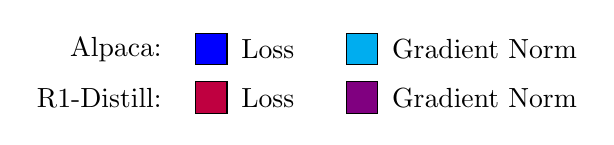
\begin{tikzpicture}
            \node[draw, fill=blue, minimum width=0.4cm, minimum height=0.4cm] (A) {};
            \node[left=0.3cm of A] {Alpaca:};
            \node[right=0.05cm of A] {Loss};

            \node[draw, fill=cyan, minimum width=0.4cm, minimum height=0.4cm, right=1.5cm of A] (B) {};
            \node[right=0.05cm of B] {Gradient Norm};

            \node[draw, fill=purple, minimum width=0.4cm, minimum height=0.4cm, below=0.2cm of A] (C) {};
            \node[left=0.3cm of C] {R1-Distill:};
            \node[right=0.05cm of C] {Loss};

            \node[draw, fill=violet, minimum width=0.4cm, minimum height=0.4cm, right=1.5cm of C] (D) {};
            \node[right=0.05cm of D] {Gradient Norm};
        \end{tikzpicture}
    }

    \caption{Training performance comparison of DeepSeek and Alpaca models.
        (a) and (b) show loss and gradient norm trends separately for each model,
        while (c) compares both losses for direct convergence analysis.}
    \label{fig:groupplot_example}
\end{figure}

% ---------------------------------------------------------
%
% DISCUSSION
%
% ---------------------------------------------------------

\section{Discussion}\label{sec:discussion}
\todo{TBD, only do if there is actual deeper meaning otherwise fuse with experiments}

\todo{Interpret the results in a deeper way:
- Why did certain methods do better?
- Mention any error analysis or interesting observations.
}

% ---------------------------------------------------------
%
% CONCLUSION
%
% ---------------------------------------------------------

\section{Conclusion and Future Work}\label{sec:conclusion-and-future-work}
\todo{TBD otherwise leave out}
\todo{Summarize the key findings and how they link back to your problem statement. Suggest improvements or next steps (e.g., new dataset, advanced fusion technique, or GNN-based approach). Highlight what you learned and what remains challenging.}

\todo{fix this}
In \cref{fig:groupplot_example} we do something very cool.\cite{hetionet}

\bibliography{main}

\end{document}
